\documentclass[a4paper,11pt,twoside,openright]{book}							% COMANDI INIZIALI
\usepackage[italian]{babel}								% sillabazione italiana
\usepackage[utf8]{inputenc}								% Per le lettere accentate IN UNIX E IN WINDOWS
\usepackage{ragged2e}					 				% giustifica
\usepackage{amsmath}									% Per allineare le equazioni
\usepackage{amssymb}									% Per le lettere dell'indicatrice (mathbb)

\usepackage{graphicx}
\usepackage{amsthm}
\usepackage{amssymb}
\usepackage{amsmath}
\usepackage{mathtools}
\usepackage{caption}
\usepackage{booktabs}
\usepackage{hyperref}
\usepackage{float}
\usepackage{subfigure}
\usepackage{multirow}
\usepackage{array}



\justifying 										% giustifica

\date{28 Luglio 2014}
\author{Gabriele Mazza}
\title{Rifiuti nella provincia di Venezia}

\begin{document}

%Indice e numerazione
\pagenumbering{arabic}

\tableofcontents

\chapter{Introduzione}
\label{Cap:intro}

Il presente lavoro di tesi illustra un modello statistico spatio-temporal spline regression (STR-PDE) per l'analisi funzionale di dati distribuiti in spazio e tempo. Quanto fatto può essere considerato un'estensione dei modelli proposti in \cite{art:sangalli}, che studiano la possibilità di costruire una stima funzionale per dati distribuiti su un dominio spaziale attraverso l'approssimazione in basi di elementi finiti. Il modello STR-PDE, invece, sviluppa una tecnica analoga permettendo la variazione temporale alla stima funzionale precedente. Di conseguenza, può essere considerato un buon strumento per lo studio di fenomeni varianti in spazio e in tempo. Dalla modellizzazione matematica è stato sviluppato un algoritmo e il codice R per il calcolo della soluzione numerica della stima.

Il lavoro è motivato dalla ricerca di un buon metodo di analisi di un dataset contenente le misurazioni della produzione dei rifiuti urbani pro capite nei comuni della provincia di Venezia tra il 1997 e il 2011. I dati sono stati raccolti ed elaborati dall'Agenzia Regionale per la Prevenzione e Protezione Ambientale del Veneto (Arpav) e sono disponibili sul sito di Open Data Veneto\footnote{\href{http://dati.veneto.it/dataset/produzione-annua-di-rifiuti-urbani-totale-e-pro-capite-1997-2011}{http://dati.veneto.it/dataset/produzione-annua-di-rifiuti-urbani-totale-e-pro-capite-1997-2011}} per la consultazione e il trattamento. Sono disponibili le misurazioni per tutta la regione del Veneto, ma per semplicità computazionale e per l'elevato interesse della laguna veneta sarà analizzata solo la provincia di Venezia. Il modello STR-PDE permette di stimare l'andamento della produzione dei rifiuti su tutta la regione e ad ogni istante di tempo nell'intervallo considerato, garantendo una chiara visualizzazione del fenomeno.

Il lavoro di tesi sarà strutturato come segue. Nel Capitolo \ref{cap:panoramica} è riportato un excursus sui metodi simili già esistenti in letteratura. Nel Capitolo \ref{cap:modello} è presentata la costruzione del modello matematico STR-PDE. Nel Capitolo \ref{cap:domC} si hanno i primi risultati, derivanti dall'applicazione del modello e del codice R al caso del dominio a forma di C descritto in \cite{art:ramsay} e \cite{art:wood}, per il quale è possibile valutare la bontà delle stime ottenute grazie alla perfetta conoscenza del fenomeno reale in ogni punto e in ogni istante. Nel capitolo \ref{cap:confronto} il modello STR-PDE è paragonato ad altri metodi già esistenti per il confronto delle stime ottenute. Nel Capitolo \ref{cap:rifiuti} si ha l'applicazione allo studio della produzione dei rifiuti nella provincia di Venezia, e infine nel Capitolo \ref{cap:conclusione} sono raccolte le conclusioni e i possibili sviluppi futuri.



\chapter{Panoramica sui modelli già esistenti}
\label{cap:panoramica}
Prima dello sviluppo del modello STR-PDE, è stato necessario uno studio dell'ambito in cui si inserisce il modello. Sono già presenti in letteratura tecniche per l'analisi funzionale di dati di questo tipo.

\chapter{Presentazione modello}
\label{cap:modello}

\chapter{Applicazione al dominio a forma di C}
\label{cap:domC}

\chapter{Confronto con gli altri modelli}
\label{cap:confronto}

Il modello STSR rappresenta una generalizzazione del caso puramente spaziale proposto in \cite{art:sangalli} e, come già evidenziato nel Capitolo \ref{cap:panoramica}, non è l'unico modello disponibile per l'analisi di dati distribuiti sia in spazio che in tempo. Pertanto è necessario che sia valutata la bontà del modello attraverso il confronto con altri metodi esistenti e studiati in letteratura, al fine di poter dire se e quanto il modello STR-PDE possa rappresentare un miglioramento in questo campo.

L'articolo \cite{art:augustin} propone l'analisi di dati di questo tipo attraverso modelli misti additivi generalizzati (GAMM) di interazione spazio-tempo. Questo metodo è generalizzato, quindi può essere usato per spiegare anche funzioni del valore atteso della risposta. Nel nostro caso, per avvicinarci al caso STR-PDE, si ipotizza che la risposta sia pari alla somma di una funzione e di un eventuale termine con covariata. Alla funzione è associato lo smoothing secondo il prodotto tensoriale dei termini marginali in spazio e tempo con le loro penalizzazioni. Quindi la costruzione dei GAMM è molto simile a quella analizzata in STR-PDE, e grazie al codice implementato nel pacchetto R \textit{mgcv} è possibile scegliere tra più tipi di modelli. In particolare ne saranno studiati due, i più simili al modello STR-PDE:
\begin{itemize}
\item TPS, in cui sono poste marginalmente \textit{cubic regression splines} in tempo e \textit{thin plate splines} in spazio;
\item SOAP, che considera \textit{cubic regression splines} in tempo e \textit{soap film smoothing} in spazio.
\end{itemize}

Un altro metodo da confrontare è sicuramente il kriging (KRIG) spazio-temporale. Le stime sono ottenute fissando un variogramma separabile e marginalmente esponenziale in spazio e tempo. I parametri dei variogrammi sono stimati dal variogramma empirico, e successivamente è possibile eseguire la stima grazie al codice implementato nel pacchetto R \textit{spacetime}.

I quattro modelli sono confrontati sull'esempio del dominio a forma di C proposto precedentemente, poichè garantisce di poter conoscere in ogni punto spaziale e ad ogni istante temporale il valore esatto della funzione. La triangolazione e i dati sono ricavati esattamente allo stesso modo di quanto fatto nel Capitolo \ref{cap:domC}. In aggiunta è stata costruita una griglia spazio-temporale di punti per la validazione: sono stati presi 80 punti equispaziati in $(-1,+3.5)$ per l'ascissa, 40 punti in equispaziati $(-1,+1)$ per l'ordinata e 20 istanti in $(0,2\pi)$ per il tempo. Ovviamente la validazione è stata studiata soltanto sui punti che ricadevano all'interno del dominio a forma di C.

I modelli sono stati confrontati attraverso il Root Mean Square Error ($\mathrm{RMSE}$) prodotto sui punti di validazione. Quindi se se $V$ è l'insieme dei punti della griglia interni al dominio, e $\mathrm{Mod}$ rappresenta la stima ottenuta dal modello, si avrà:
$$
\mathrm{RMSE}_V(\mathrm{Mod})=\sqrt{\frac{\sum_{(\underline p_i,t_i)\in V} (\mathrm{Mod}(\underline p_i,t_i)-g(\underline p_i)cos(t_i))^2}{\mathrm{card}(V)}}
$$ 

Il procedimento è stato iterato 50 volte, per poter escludere possibili andamenti particolari dovuti alla generazione del rumore.
 
\begin{figure}[t]
	\centering
	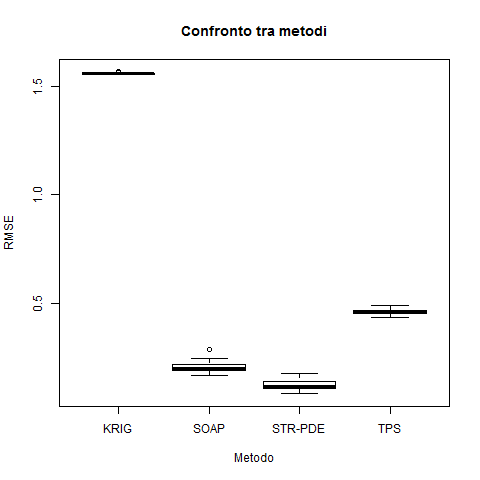
\includegraphics[width=0.60\textwidth]{Immagini/Confronto_metodi.png}   
	\caption{Confronto del $\mathrm{RMSE}$, caso senza covariate}
	\label{fig:cfr}
\end{figure}
Nel caso senza covariate si hanno i risultati riportati in figura \ref{fig:cfr}. Sono stati tracciati i boxplot dei valori di $\mathrm{RMSE}$ calcolati nelle 50 iterazioni per ogni metodo. Si hanno alti valori per KRIG e TPS (e questo fa presupporre una stima non buona), ma il modello che commette meno errore è STR-PDE.

AGGIUNTA DEI GRAFICI..

\chapter{Produzione di rifiuti nella provincia di Venezia}
\label{cap:rifiuti}



\chapter{Conclusioni e sviluppi futuri}
\label{cap:conclusione}

In questo lavoro di tesi è stato analizzato nel dettaglio il modello STR-PDE nell'ambito della stima funzionale per dati varianti all'interno di un dominio spaziale e di un intervallo temporale. Il modello, che si propone di essere un'estensione del caso puramente spaziale già analizzato in letteratura, è stato sviluppato in codice R. Dal confronto con gli altri metodi e da quanto ricavato con le stime, soprattutto sul dominio a forma di C in cui è possibile conoscere il valore reale della funzione, si può concludere che i risultati prodotti sono molto buoni.

Diversa è la conclusione per le prestazioni computazionali del codice. Per semplicità computazionale le basi degli elementi finiti sono state scelte lineari e la produzione dei rifiuti è stata analizzata solamente nella provincia di Venezia, pur avendo a disposizione i dati di tutto il Veneto. Inoltre, durante l'esecuzione del codice, si è potuto notare che alcune funzioni come la minimizzazione di $\mathrm{GCV}(\underline \lambda)$ o il calcolo dei valori stimati ad un istante di tempo fissato (usati ad esempio per conoscere il profilo della funzione ad un certo anno) sono molto lente. Ovviamente per analisi di dataset di grosse dimensioni deve essere messa in conto una spesa di tempo elevata, ma R certamente non ha aiutato. Infatti, è noto che R non sia un linguaggio di programmazione fortemente efficiente, e questo ha caratterizzato la lentezza di esecuzione. Il più chiaro sviluppo futuro può essere l'uso di questo codice come base per lo sviluppo di un algoritmo più veloce, attraverso l'integrazione con un linguaggio di programmazione più efficiente (come il C++) nei colli di bottiglia più evidenti.

Dopo che sarà stata sviluppata l'integrazione del codice, sarà possibile garantire una analisi più agile anche per dataset di dimensioni più elevate o per elementi finiti di ordine maggiore. In questo modo si avrà a disposizione uno strumento di analisi statistica buono non solo dal punto di vista dei risultati, ma anche in termini di efficienza computazionale.


\begin{thebibliography}{9}

\bibitem{art:augustin}
Nicole H. Augustin, Verena M. Trenkel, Simon N. Wood, Pascal Lorance, \emph{Space-time modelling of blue ling for fisheries stock management}, Environmetrics, 24, 109–119, (2013)

\bibitem{art:azzimonti}
Laura Azzimonti, Laura M. Sangalli, Piercesare Secchi, Maurizio Domanin, Fabio Nobile, \emph{Blood flow velocity field estimation via spatial regression with PDE penalization}, Journal of the American Statistical Association, (2015)

\bibitem{art:gcv}
Peter Craven, Grace Wahba, \emph{Smoothing noisy data with spline functions: estimating the correct degree of smoothing by the method of generalized cross-validation}, Numerische Mathematik, 31, 377–403, (1979)

\bibitem{art:marra}
Giampiero Marra, David L. Miller, Luca Zanin, \emph{Modelling the spatiotemporal distribution of the incidence of resident foreign population}, Statistica Neerlandica, 66, 133–160, (2012)

\bibitem{art:ramsay}
Timothy O. Ramsay, \emph{Spline smoothing over difficult regions}, Journal of the Royal Statistical Society: Series B, 64, 307–319, (2002)

\bibitem{art:sangalli}
Laura M. Sangalli, James O. Ramsay, Timothy O. Ramsay, \emph{Spatial spline regression models}, Journal of the Royal Statistical Society: Series B, 75, 681–703, (2013)

\bibitem{art:wood}
Simon N. Wood, Mark W. Bravington, Sharon L. Hedley, \emph{Soap film smoothing}, Journal of the Royal Statistical Society: Series B, 70, 931–955, (2008)


%\bibitem{prog:R}
%R Core Team, \emph{R: A Language and Environment for Statistical Computing}, R Foundation for Statistical Computing, Vienna, 2013, \url{http://www.R-project.org/}

\end{thebibliography}


\end{document}
